\chapter{System Analysis}

The project hosts two kinds of users: admin and users. 

The user will start a trip, save location and media, manipulate media share options and share all of contents on social media. Also user can download a shared content which that user has access privileges. User can follow the trip that downloaded. User can search other users; trips by location, name and trip type (walk, run, ride or car). User can organize team trips with other users. During the team trip users can see each other's location on the map.

The admin **TARIK BURAYI SEN YAZ**.

The work model of the system is shown in Figure~\ref{fig:system_diagram}.

\begin{figure}[!htbp]
\centering
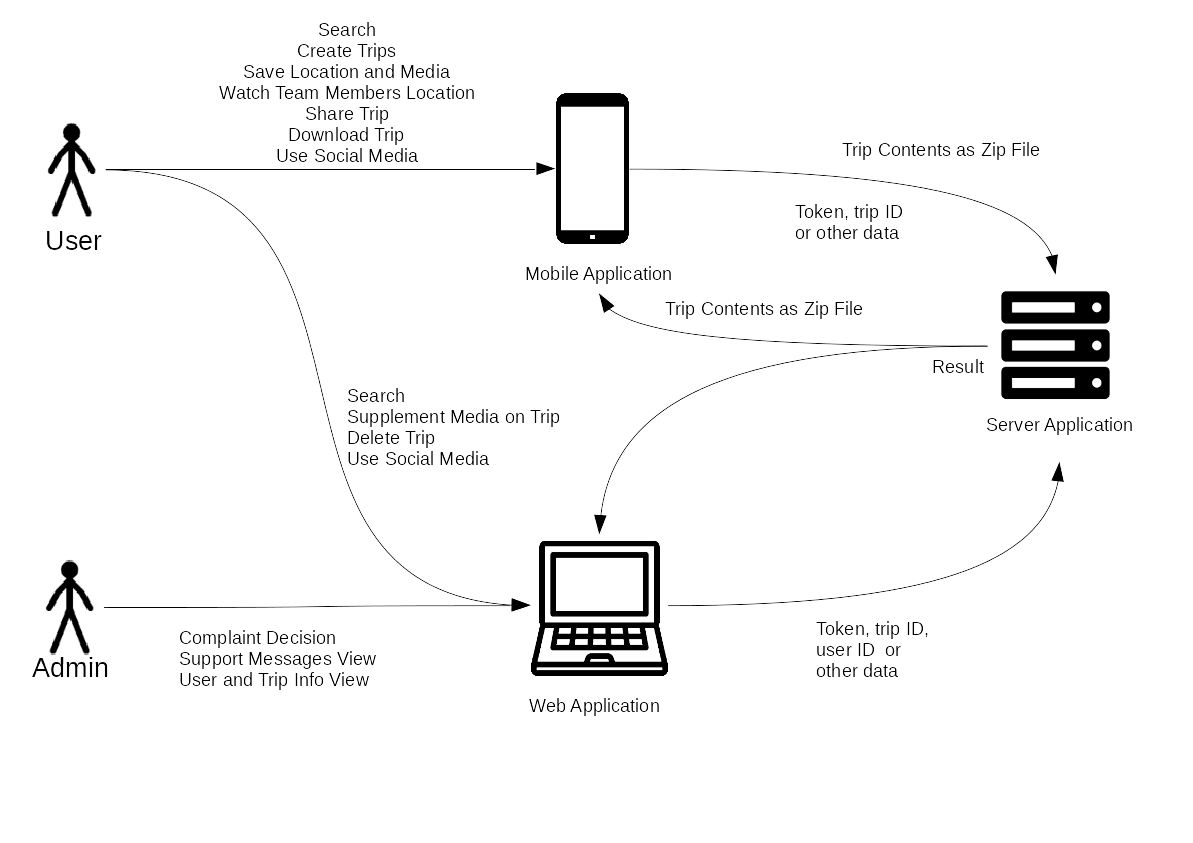
\includegraphics[width=\textwidth]{projectChapters/images/system_diagram.png}
\caption{System Schema}
\label{fig:system_diagram}
\end{figure}

\begin{figure}[!htbp]
\centering
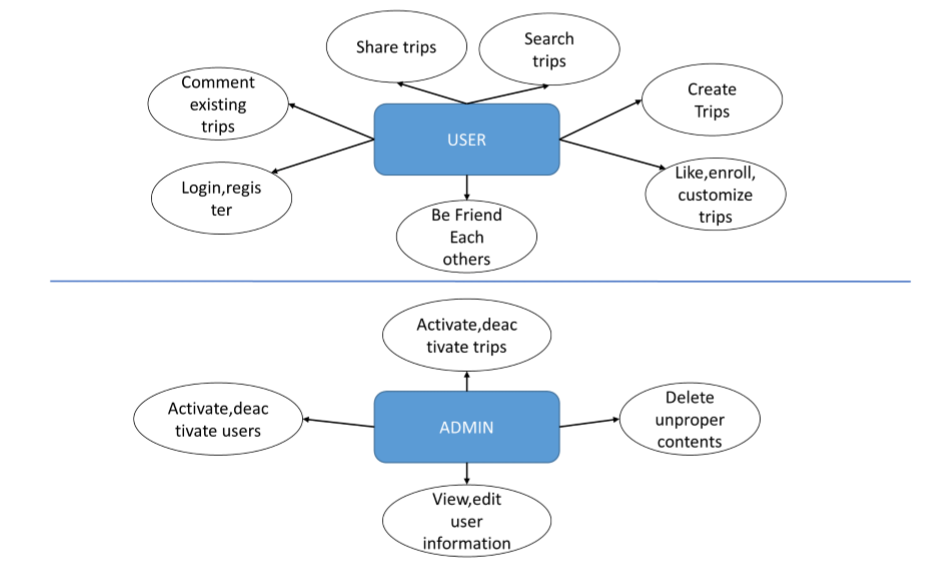
\includegraphics[width=\textwidth]{projectChapters/images/ER.png}
\caption{User Roles}
\label{fig:roles}
\end{figure}